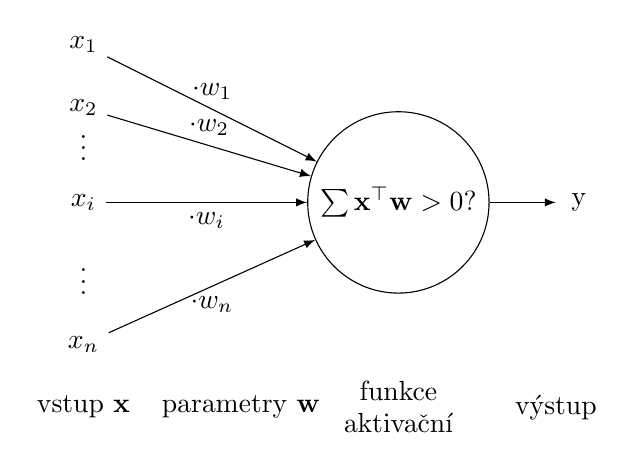
\begin{tikzpicture}[]

\tikzset{>=latex}
\def\inputX{-4.0}
\def\labelY{-2.6}

\draw (0,\labelY - 0.2) node {aktivační};
\draw (0,\labelY + 0.2) node {funkce};

\draw (\inputX,\labelY) node {vstup $\mathbf{x}$};

\draw (\inputX / 2,\labelY) node {parametry $\mathbf{w}$};

\draw (2.0, \labelY) node {výstup};


\draw (0,0) node[draw,circle](neuron) {$\sum \mathbf{x}^\top\mathbf{w} > 0$?};
    \draw[->] (neuron) -- (2,0) node {~~~~~y};

\draw (\inputX,0) node {$x_i$} edge[->] node[anchor=north, pos=.5] {$\cdot w_i$} (neuron);

\draw (\inputX,2.0) node {$x_1$} edge[->]
    node[anchor=south, pos=.5] {$\cdot w_1$} (neuron);
\draw (\inputX,1.2) node {$x_2$} edge[->]
    node[anchor=south, pos=.5] {$\cdot w_2$} (neuron);

\draw (\inputX,0.8) node {$\vdots$};

\draw (\inputX,-0.9) node {$\vdots$};

\draw (\inputX,-1.8) node {$x_n$} edge[->]
    node[anchor=north, pos=.5, below] {$\cdot w_n$} (neuron);

\end{tikzpicture}
